\chapter{Balanced Clustering} 
\label{chap:balance}

In this chapter, we examine the reasons that cause load imbalance in task clustering. Furthermore, we propose a series of balanced task clustering methods to address these imbalance problems. A trace-based simulation shows our methods can significantly improve the runtime performance of five widely used workflows compared to the na\"{i}ve implementation of task clustering.

\section{Motivation}


Existing task clustering strategies have demonstrated their effect in some scientific workflows such as CyberShake \cite{Rynge2012} and LIGO \cite{Deelman2002}. However, there are several challenges that are not yet addressed. 

The first challenge users face when executing workflows is task runtime variation. 
%Tasks may have diverse task runtimes and such diversity may cause some load imbalance. The last completed task among a given set of tasks essentially controls the release of next set of tasks. 
In a scientific workflow, tasks within a level (or depth within a workflow directed acyclic graph) may have different runtimes. Merging tasks within a level without considering the runtime variance may cause load imbalance, i.e., some clustered jobs may be composed of short running tasks while others of long running tasks. This imbalance delays the release of tasks from the next level of the workflow, penalizing the workflow execution with an overhead produced by the use of inappropriate task clustering strategies.
A common technique to handle load imbalance is overdecomposition~\cite{Lifflander2012}.
This method decomposes computational work into medium-grained balanced tasks. Each task is coarse-grained enough to enable efficient execution and reduce scheduling overheads, while being fine-grained enough to expose significantly higher application-level parallelism than what is offered by the hardware. 

The second challenge deals with the complex data dependencies within a workflow. 
Merging tasks that have no intermediate data between them seems safe at the first sight. However, the subsequent tasks that rely on the output data that their parent tasks produce may suffer a data locality problem since data may be distributed poorly and the data transfer time is increased.  As a result, data transfer times and failure probabilities increase. Therefore, we claim that data dependencies of subsequent tasks should be considered.


%We generalize these two challenges (Runtime Imbalance and Dependency Imbalance) to the general imbalance problem. It means that the execution of workflows suffers from significant overheads (unavailable data, overloaded resources, or system constraints) due to inappropriate task clustering and job execution. To solve the imbalance problem, we introduce a series of balancing methods to address these two challenges respectively. 
%This is from FGCS
We generalize these two challenges (Runtime Imbalance and Dependency Imbalance) to the general load balance problem. We introduce a series of balancing methods to address these challenges. However, there is a tradeoff between runtime and data dependency balancing. For instance, balancing runtime may aggravate the Dependency Imbalance problem, and vice versa. Therefore, we propose a series of quantitative metrics that reflect the internal structure (in terms of task runtimes and dependencies) of the workflow and use them as a criterion to select and balance these solutions.

%However, what makes this problem challenging is that the solutions are usually conflicting. For example, balancing runtime may worsen the Dependency Imbalance problem, and vice versa. A quantitative measurement of workflow characteristics is required to serve as a criterion to select and balance these solutions. To achieve this goal, we propose four metrics to reflect the internal structure (in terms of runtime and dependency) of the workflow. 

In particular, we provide a novel approach to capture these metrics. Traditionally, there are two approaches to improve the performance of task clustering. The first one is a top-down approach \cite{Integration2012} that represents the task clustering problem as a global optimization problem and aims to minimize the overall runtime of a workflow. However, the complexity of solving such an optimization problem does not scale well. The second one is a bottom-up approach \cite{Muthuvelu2005}\cite{Liu2009} that only examines free tasks to be merged and optimizes the task clustering results locally. In contrast, our work extends these solutions to consider the neighboring tasks including siblings, parents, children and so on because such a family of tasks has strong connections between them. 

%The third contribution we make is that we analyze and connect the performance of these metrics and balancing methods. These quantitative metrics indicate which type of imbalance problem a workflow is more likely to suffer from. Comparing the relative values of these metrics informs the selection of a balancing method or a combination of these methods. 
In this chapter, we address the balancing problem by studying (\emph{i}) the performance gain of using our balancing methods over a baseline execution on a larger set of workflows; (\emph{ii}) the performance gain over two additional task clustering methods in literature; (\emph{iii}) the performance impact of the variation of the average data size and the number of resources; and (\emph{iv}) the performance impact of combining our balancing methods with vertical clustering.


\section{Related Work}
\textbf{Workflow Scheduling}. There have been a considerable amount of work trying to solve workflow-mapping problem using DAG scheduling heuristics such as HEFT \cite{Topcuoglu2002}, Min-Min \cite{Blythe2005}, MaxMin \cite{Braun2001}, MCT \cite{Braun2001}, etc. Duan \cite{Rubing2005} and Wieczorek \cite{Wieczorek2005} have discussed the scheduling and the partitioning of scientific workflows in dynamic grids. The emergence of cloud computing \cite{Armbrust2009} has made it possible to easily lease large-scale homogeneous computing resources from commercial resource providers and satisfy QoS requirements. In our case, since we assume resources are homogeneous, the resource selection is not a major concern and thus the scheduling problem can be simplified as a task clustering problem. 
More specifically, a plethora of  scheduling algorithms have been developed in the networking and operating system domains. Many of these schedulers have been extended to perform in a hierarchical fashion~\cite{Lifflander2012}, which divides the tasks into independent autonomous groups and organizes the groups in a hierarchy. Lifflander et al.~\cite{Lifflander2012} proposed to use work stealing and a hierarchical persistence-based rebalancing algorithm to address the imbalance problem in scheduling. Zheng et al.~\cite{Zheng2011} presented an automatic hierarchical load balancing method that overcomes the scalability challenges of centralized schemes and poor solutions of traditional distributed schemes. There are other scheduling algorithms~\cite{Braun2001} (e.g. list scheduling) that indirectly achieve load balancing of workflows through makespan minimization. However, the benefit that can be achieved through traditional scheduling optimization is limited by its complexity. The performance gain of task clustering is primarily determined by the ratio between system overheads and task runtime, which is more substantial in modern distributed systems such as clouds and grids. 

\textbf{Task Granularity Control} has also been addressed in scientific workflows. For instance, Singh et al.~\cite{Singh2008} proposed a level- and label-based clustering. In level-based clustering, tasks at the same workflow level can be clustered together. The number of clusters or tasks per cluster is specified by the user. In the label-based clustering, the user labels tasks that should be clustered together. Although their work considers data dependencies between workflow levels, it is done manually by the users, a process that is prone to errors. Recently, Ferreira da Silva et al.~\cite{Ferreira-granularity-2013} proposed task grouping and ungrouping algorithms to control workflow task granularity in a non-clairvoyant and online context, where none or few characteristics about the application or resources are known in advance. Their work significantly reduced scheduling and queuing time overheads, but did not consider data dependencies. The low performance of \emph{fine-grained} tasks is a common problem in widely distributed platforms where the scheduling overhead and queuing times at resources are high, such as grid and cloud systems. Several works have addressed the control of task granularity of bags of tasks. For instance, Muthuvelu et al.~\cite{Muthuvelu2005} proposed a clustering algorithm that groups bags of tasks based on their runtime---tasks are grouped up to the resource capacity. Later, they extended their work~\cite{4493929} to determine task granularity based on task file size, CPU time, and resource constraints. Recently, they proposed an online scheduling algorithm~\cite{Muthuvelu2010,Muthuvelu2013} that groups tasks based on resource network utilization, user's budget, and application deadline. Ng et al.~\cite{Keat2006} and Ang et al.~\cite{Ang2009} introduced bandwidth in the scheduling framework to enhance the performance of task scheduling. Longer tasks are assigned to resources with better bandwidth. Liu and Liao~\cite{Liu2009} proposed an adaptive fine-grained job scheduling algorithm to group fine-grained tasks according to processing capacity and bandwidth of the current available resources. Although these techniques significantly reduce the impact of scheduling and queuing time overhead, they did not consider data dependencies.

\textbf{Load Balancing.} With the aim of dynamically balancing the computational load among resources, some jobs have to be moved from one resource to another and/or from one period of time to another, which is called task reallocation \cite{Tomas2012}. Caniou  \cite{Caniou2011} presented a reallocation mechanism that tunes parallel jobs each time they are submitted to the local resource manager. They only needed to query batch schedulers with simple submission or cancellation requests. They also presented different reallocation algorithms and studied their behavior in the case of a multi-cluster environment. In \cite{Zhang2000}, a preemptive process migration method was proposed to dynamically migrate processes from overloaded computational nodes to lightly-loaded nodes. However, this approach can achieve a good balance only when there are some idle compute nodes (e.g. when the number of task processes is less than that of compute nodes). In our case, since we deal with large-scale scientific workflows, usually we have more tasks than available compute nodes. 
Guo et al. \cite{Zhenhua2011} presented mechanisms to dynamically split and consolidate tasks to cope with load imbalance. They have proposed algorithms to dynamically split unfinished tasks to fill idle compute nodes. Similarly, Ying et al. \cite{Ying2009} proposed a load-balancing algorithm based on collaborative task clustering. The algorithm divides the collaborative computing tasks into subtasks and then dynamically allocates them to the servers. Compared to these approaches, our work selects tasks to be merged based on their task runtime distribution and their data dependencies initially, without introducing additional overheads during the runtime. Also, a quantitative approach of imbalance measurement guides the selection of tasks to be merged without causing runtime imbalance or dependency imbalance. 

\section{Approach}


 In this section, we introduce metrics that quantitatively capture workflow characteristics to measure runtime and dependence imbalances. We then present methods to address the load balance problem.



\subsection{Imbalance metrics}

\textbf{Runtime Imbalance} describes the difference of the task/job runtime of a group of tasks/jobs. In this work, we denote the \textbf{Horizontal Runtime Variance} ($HRV$) as the ratio of the standard deviation in task runtime to the average runtime of tasks/jobs at the same horizontal level of a workflow. At the same horizontal level, the job with the longest runtime often controls the release of the next level jobs. A high $HRV$ value means that the release of next level jobs has been delayed. Therefore, to improve runtime performance, it makes sense to reduce the standard deviation of job runtime. Figure~\ref{fig:imbalance_rv} shows an example of four independent tasks $t_1$, $t_2$, $t_3$ and $t_4$ where the task runtime of $t_1$ and $t_2$ is 10 seconds, and the task runtime of $t_3$ and $t_4$ is 30 seconds. In the Horizontal Clustering (HC) approach, a possible clustering result could be merging $t_1$ and $t_2$ into a clustered job, and $t_3$ and $t_4$ into another. This approach results in imbalanced runtime, i.e., $HRV > 0$ (Figure~\ref{fig:imbalance_rv}-top). In contrast, a balanced clustering strategy should try its best to evenly distribute task runtime among jobs as shown in Figure~\ref{fig:imbalance_rv} (bottom). A smaller \emph{HRV} means that the runtime of tasks within a horizontal level is more evenly distributed and therefore it is less necessary to use runtime-based balancing algorithms. However, runtime variance is not able to describe how symmetric the structure of the dependencies between tasks is.

\begin{figure}[htb]
	\centering
	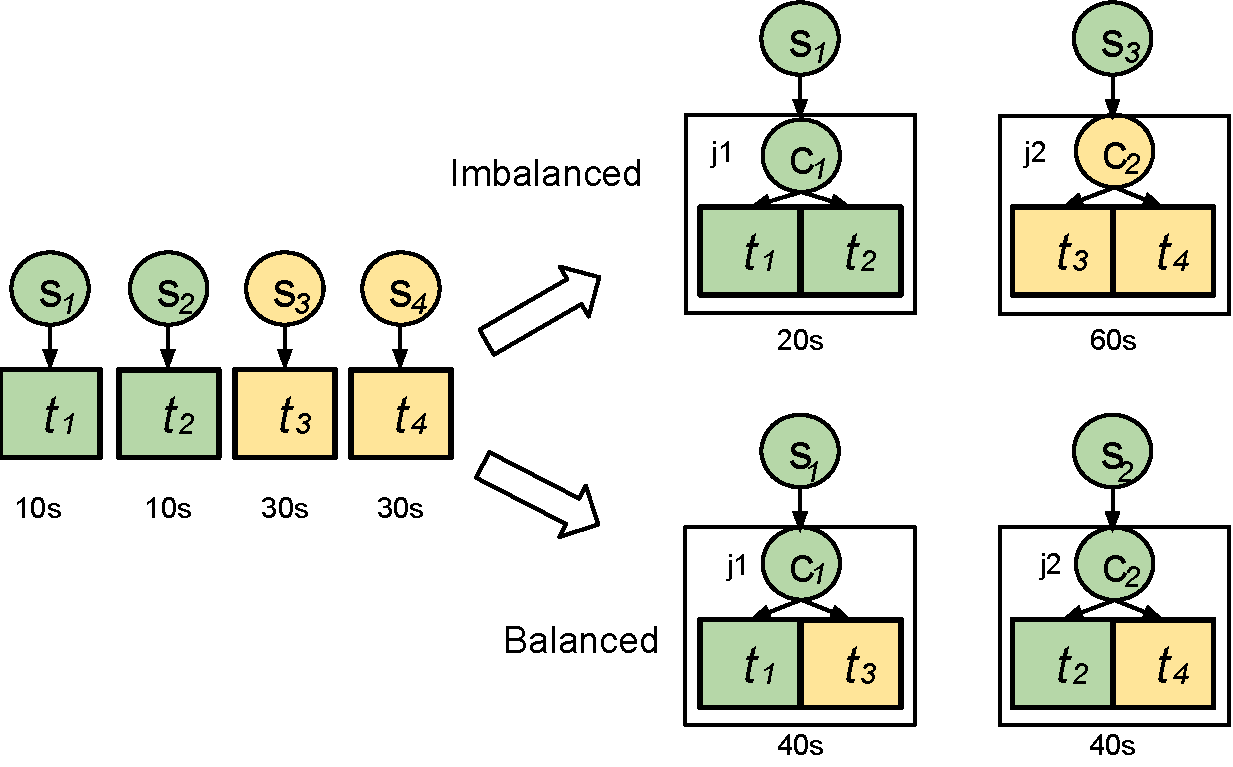
\includegraphics[width=0.8\linewidth]{figures/balance/figure5.pdf}
	\captionof{figure}{An example of Horizontal Runtime Variance.}
	\label{fig:imbalance_rv}
\end{figure}


\textbf{Dependency Imbalance} means that the task clustering at one horizontal level forces the tasks at the next level (or even subsequent levels) to have severe data locality problems and thus loss of parallelism. For example, in Figure~\ref{fig:imbalance_dv}, we show a two-level workflow composed of four tasks in the first level and two in the second. Merging $t_1$ with $t_3$ and $t_2$ with $t_4$ (imbalanced workflow in Figure~\ref{fig:imbalance_dv}) forces $t_5$ and $t_6$ to transfer files from two locations and wait for the completion of $t_1$, $t_2$, $t_3$, and $t_4$.  A balanced clustering strategy groups tasks that have the maximum number of child tasks in common. Thus, $t_5$ can start to execute as soon as $t_1$ and $t_2$ are completed, and so can $t_6$. To measure and quantitatively demonstrate the Dependency Imbalance of a workflow, we propose two  metrics: ($i$) Impact Factor Variance, and ($ii$) Distance Variance. 

\begin{figure}[htb]
	\centering
	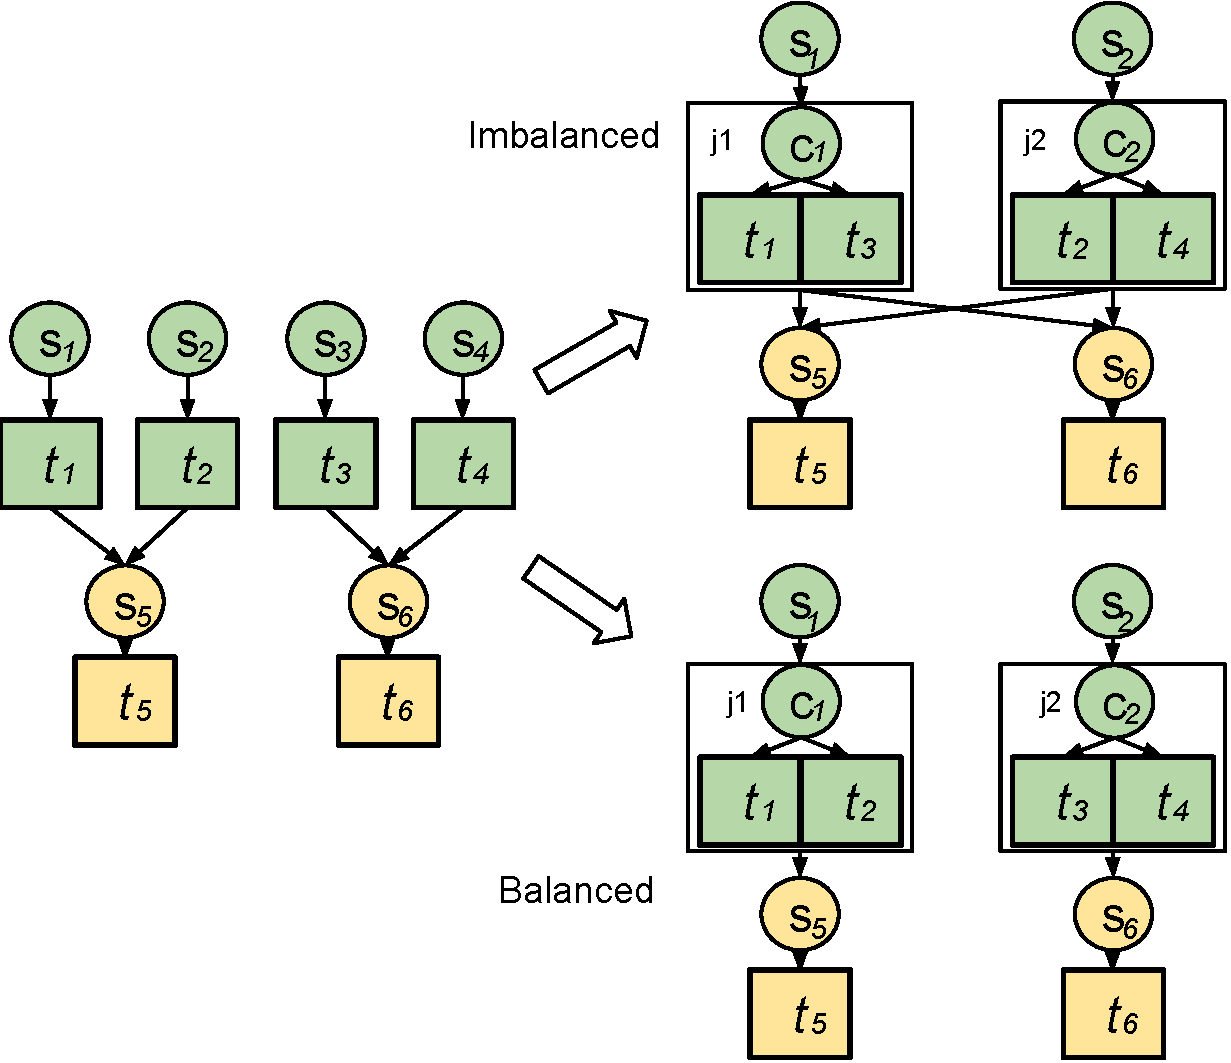
\includegraphics[width=0.8\linewidth]{figures/balance/figure6.pdf}
	\captionof{figure}{An example of Dependency Imbalance.}
	\label{fig:imbalance_dv}
\end{figure}

We define the \textbf{Impact Factor Variance} ($IFV$) of tasks as the standard deviation of their impact factors. The \textbf{Impact Factor} ($IF$) of a task $t_u$ is defined as follows:

\begin{equation}
\label{eq:imbalance_impact_factor}
	IF(t_u)=\sum_{t_v\in Child(t_u)}^{}\frac{IF(t_v)}{||Parent(t_v)||}
\end{equation}
where $Child(t_u)$ denotes the set of child tasks of $t_u$, and $||Parent(t_v)||$ the number of parent tasks of $t_v$. The Impact Factor aims at capturing the similarity of tasks/jobs in a graph by measuring their relative impact factor or importance to the entire graph. Tasks with similar impact factors are merged together, so that the workflow structure tends to be more `even' or symmetric. For simplicity, we assume the $IF$ of a workflow exit task (e.g. $t_5$ in Figure~\ref{fig:imbalance_dv}) is 1.0. For instance, consider the two workflows presented in Figure~\ref{fig:imbalance_hifv}. The $IF$ for each of $t_1$, $t_2$, $t_3$, and $t_4$ is computed as follows:

\begin{eqnarray*}
	\displaystyle  
	&IF(t_7 )=1.0, IF(t_6 )=IF(t_5 )=IF(t_7 )/2=0.5\nonumber  \\
	&IF(t_1 )=IF(t_2 )=IF(t_5 )/2=0.25\nonumber \\
	&IF(t_3 )=IF(t_4 )=IF(t_6 )/2=0.25\nonumber 
\end{eqnarray*}

Thus, IFV($t_1$, $t_2$, $t_3$, $t_4$) = 0. In contrast, the $IF$ for $t_{1'}$, $t_{2'}$, $t_{3'}$, and $t_{4'}$ is:

\begin{eqnarray*}
	\displaystyle  
	&IF(t_{7'})=1.0, IF(t_{6'})=IF(t_{5'})=IF(t_{1'})=IF(t_{7'})/2=0.5\nonumber \\
	&IF(t_{2'})=IF(t_{3'})=IF(t_{4'})=IF(t_{6'})/3=0.17 \nonumber
\end{eqnarray*}

Therefore, the $IFV$ value for {$t_{1'}$, $t_{2'}$, $t_{3'}$, $t_{4'}$} is 0.17, which predicts it is likely to be less symmetric than the workflow in Figure~\ref{fig:imbalance_hifv} (left). In this chapter, we use \textbf{HIFV} (Horizontal IFV) to indicate the $IFV$ of tasks at the same horizontal level. The time complexity of calculating the $IF$ of all the tasks of a workflow with $n$ tasks is $O(n)$.  

\begin{figure}[htb]
	\centering
	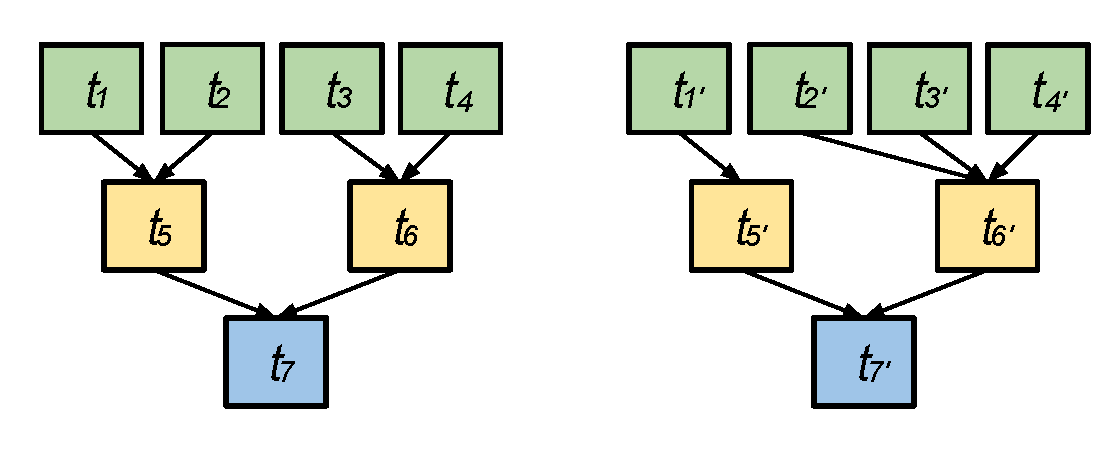
\includegraphics[width=0.75\linewidth]{figures/balance/figure7.pdf}
	\captionof{figure}{Example of workflows with different data dependencies}
	\label{fig:imbalance_hifv}
\end{figure}

\textbf{Distance Variance} ($DV$) describes how `close' tasks are to each other. The distance between two tasks/jobs is defined as the cumulative length of the path to their closest common successor. If they do not have a common successor, the distance is set to infinity. For a group of $n$ tasks/jobs, the distance between them is represented by a $n \times n$ matrix $D$, where an element $D(u,v)$ denotes the distance between a pair of tasks/jobs $u$ and $v$. For any workflow structure, $D(u,v)=D(v,u)$ and $D(u,u)=0$, thus we ignore the cases when $u \geq v$. Distance Variance is then defined as the standard deviation of all the elements $D(u,v)$ for $u<v$. The time complexity of calculating all the values of $D$ of a workflow with $n$ tasks is $O(n^2)$. 

Similarly, $HDV$ indicates the $DV$ of a group of tasks/jobs at the same horizontal level. For example, Table~\ref{tab:imblance_metric} shows the distance matrices of tasks from the first level for both workflows of Figure~\ref{fig:imbalance_hifv} ($D_1$ for the workflow in the left, and $D_2$ for the workflow in the right). $HDV$ for $t_1, t_2, t_3$, and $t_4$ is 1.03, and for $t_{1'}, t_{2'}, t_{3'}$, and $t_{4'}$ is 1.10. In terms of distance variance, $D_1$ is more `even' than $D_2$. A smaller $HDV$ means that the tasks at the same horizontal level are more equally `distant' from each other and thus the workflow structure tends to be more `even' and symmetric. 

\begin{table}[htb]
	\footnotesize
	\centering
	\begin{tabular}{l|rrrr}
		$D_1$ & $t_1$ & $t_2$ & $t_3$ &$t_4$\\
		\hline
		$t_1$ & 0 & 2 & 4 & 4 \\
		$t_2$ & 2 & 0 & 4 & 4 \\
		$t_3$ & 4 & 4 & 0 & 2\\
		$t_4$ & 4 & 4 & 2 & 0 \\
	\end{tabular}
	\quad
	\begin{tabular}{l|rrrr}
		$D_2$ & $t_1'$ & $t_2'$ & $t_3'$ &$t_4'$\\
		\hline
		$t_1'$ & 0 & 4 & 4 & 4 \\
		$t_2'$ & 4 & 0 & 2 & 2 \\
		$t_3'$ & 4 & 2 & 0 & 2\\
		$t_4'$ & 4 & 2 & 2 & 0 \\
	\end{tabular}
	\caption{Distance matrices of tasks from the first level of workflows in Figure~\ref{fig:imbalance_hifv}.}
	\label{tab:imblance_metric}
\end{table}

In conclusion, runtime variance and dependency variance offer a quantitative and comparable tool to measure and evaluate the internal structure of a workflow. 



\subsection{Balanced clustering methods}
\label{sec:balance:methods}
In this subsection, we introduce our balanced clustering methods used to improve the runtime and dependency balance in task clustering. We first introduce the basic runtime-based clustering method, and then two other balancing methods that address the dependency imbalance problem. 

\begin{algorithm}[!htb]
	\footnotesize
	\caption{Horizontal Runtime Balancing algorithm.}
	\label{alg:imbalance_hrb}
	\begin{algorithmic}[1]
		\Require $W$: workflow; $C$: number of tasks per jobs; $R$: number of jobs per horizontal level
		\Procedure{Clustering}{$W,C$}
			\For{$level < depth(W)$}
				\State $TL\gets $\ \Call{GetTasksAtLevel}{$W,level$} \Comment{Partition $W$ based on depth}
				\State $CL\gets$  \ \Call{Merge}{$TL,C, R$} \Comment{Returns a list of clustered jobs}
				\State $W \gets W - TL + CL$  \Comment{Merge dependencies as well} 
			\EndFor
		\EndProcedure
		\Procedure{Merge}{$TL, C, R$}
			\For{$i<R$}
			\State $J_i\gets$\{\}\Comment{An empty job}
			\EndFor
			\State $CL\gets$\{\}\Comment{An empty list of clustered jobs}
			\State Sort $TL$ in descending of runtime
			\ForAll{$t$ in $TL$}
				\State $J\gets$ the job with shortest runtime and less than $C$ tasks  
				\State $J$.add ($t$) \Comment{Adds the task to the shortest job}
				
			\EndFor
			\For{$i<R$}
			\State  $CL$.add( $J_i$)
			\EndFor
			\State \textbf{return} $CL$
		\EndProcedure
	\end{algorithmic}
\end{algorithm}



\textbf{Horizontal Runtime Balancing} (HRB) aims to evenly distribute task runtime among clustered jobs. Tasks with the longest runtime are added to the job with the shortest runtime. Algorithm~\ref{alg:imbalance_hrb} shows the pseudocode of HRB. This greedy method is used to address the load balance problem caused by runtime variance at the same horizontal level. Figure~\ref{fig:imbalance_hrb} shows an example of HRB where tasks in the first level have different runtimes and should be grouped into two jobs. HRB sorts tasks in decreasing order of runtime, and then adds the task with the highest runtime to the group with the shortest aggregated runtime. Thus, $t_1$ and $t_3$, as well as $t_2$ and $t_4$ are merged together.
For simplicity, system overheads are not displayed.

\begin{figure}[htb]
	\centering
	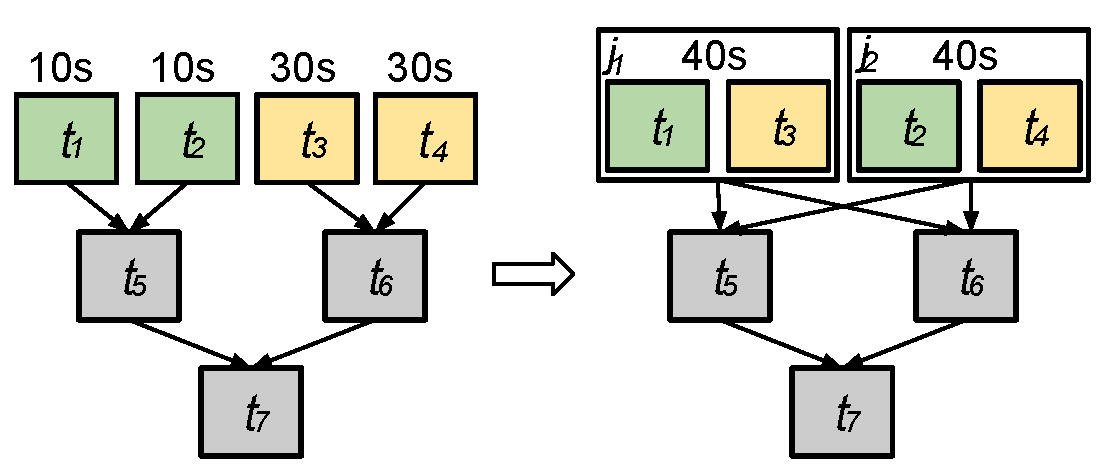
\includegraphics[width=0.7\linewidth]{figures/balance/figure8.pdf}
	\caption{An example of the HRB (Horizontal Runtime Balancing) method. By solely addressing runtime variance, data locality problems may arise.}
	\label{fig:imbalance_hrb}
\end{figure}

\begin{algorithm}[!htb]
	\footnotesize
	\caption{Horizontal Impact Factor Balancing algorithm.}
	\label{alg:imbalance_hifb}
	\begin{algorithmic}[1]
		\Require $W$: workflow; $C$: number of tasks per jobs; $R$: number of jobs per horizontal level
		\Procedure{Clustering}{$W,C$}
			\For{$level < depth(W)$}
				\State $TL\gets $\ \Call{GetTasksAtLevel}{$W,level$} \Comment{Partition $W$ based on depth}
				\State $CL\gets$  \ \Call{Merge}{$TL,C, R$} \Comment{Returns a list of clustered jobs}
				\State $W \gets W - TL + CL$  \Comment{Merge dependencies as well} 
			\EndFor
		\EndProcedure
		\Procedure{Merge}{$TL, C, R$}
			\For{$i<R$}
			\State $J_i\gets$\{\}\Comment{An empty job}
			\EndFor
			\State $CL\gets$\{\}\Comment{An empty list of clustered jobs}
			\State Sort $TL$ in descending of runtime
			\ForAll{$t$ in $TL$}
				\State $L\gets$ Sort all $J_i$ with the similarity of impact factors with $t$
				\State $J\gets$ the job with shortest runtime and less than $C$ tasks in $L$
				\State $J$.add ($t$) 
				
			\EndFor
			\For{$i<R$}
			\State  $CL$.add( $J_i$)
			\EndFor
			\State \textbf{return} $CL$
		\EndProcedure
	\end{algorithmic}
\end{algorithm}


\begin{algorithm}[!htb]
	\footnotesize
	\caption{Horizontal Distance Balancing algorithm.}
	\label{alg:imbalance_hdb}
	\begin{algorithmic}[1]
		\Require $W$: workflow; $C$: number of tasks per jobs; $R$: number of jobs per horizontal level
		\Procedure{Clustering}{$W,C$}
			\For{$level < depth(W)$}
				\State $TL\gets $\ \Call{GetTasksAtLevel}{$W,level$} \Comment{Partition $W$ based on depth}
				\State $CL\gets$  \ \Call{Merge}{$TL,C, R$} \Comment{Returns a list of clustered jobs}
				\State $W \gets W - TL + CL$  \Comment{Merge dependencies as well} 
			\EndFor
		\EndProcedure
		\Procedure{Merge}{$TL, C, R$}
			\For{$i<R$}
			\State $J_i\gets$\{\}\Comment{An empty job}
			\EndFor
			\State $CL\gets$\{\}\Comment{An empty list of clustered jobs}
			\State Sort $TL$ in descending of runtime
			\ForAll{$t$ in $TL$}
				\State $L\gets$ Sort all $J_i$ with the closest distance with $t$
				\State $J\gets$ the job with shortest runtime and less than $C$ tasks in $L$
				\State $J$.add ($t$) 
				
			\EndFor
			\For{$i<R$}
			\State  $CL$.add( $J_i$)
			\EndFor
			\State \textbf{return} $CL$
		\EndProcedure
	\end{algorithmic}
\end{algorithm}


%how HRB works in an example of four jobs with different job runtime (assuming the height of a job is its runtime). For the given task ($t_0$), HRB sorts the potential jobs ($j_1$, $j_2$, $j_3$, and $j_4$) based on their runtime and selects the shortest job (in this case $j_1$ or $j_2$). 



However, HRB may cause a dependency imbalance problem since the clustering does not take data dependency into consideration. To address this problem, we propose the \textbf{Horizontal Impact Factor Balancing} (HIFB) and the \textbf{Horizontal Distance Balancing} (HDB) methods. 

In HRB, candidate jobs within a workflow level are sorted by their runtime, while in HIFB jobs are first sorted based on their similarity of $IF$, then on runtime. 
Algorithm~\ref{alg:imbalance_hifb} shows the pseudocode of HIFB. 
For example, in Figure~\ref{fig:imbalance_hifb}, $t_1$ and $t_2$ have $IF = 0.25$, while $t_3$, $t_4$, and $t_5$ have $IF = 0.16$. HIFB selects a list of candidate jobs with the same $IF$ value, and then HRB is performed to select the shortest job. Thus, HIFB merges $t_1$ and $t_2$ together, as well as $t_3$ and $t_4$.

\begin{figure}[htb]
	\centering
	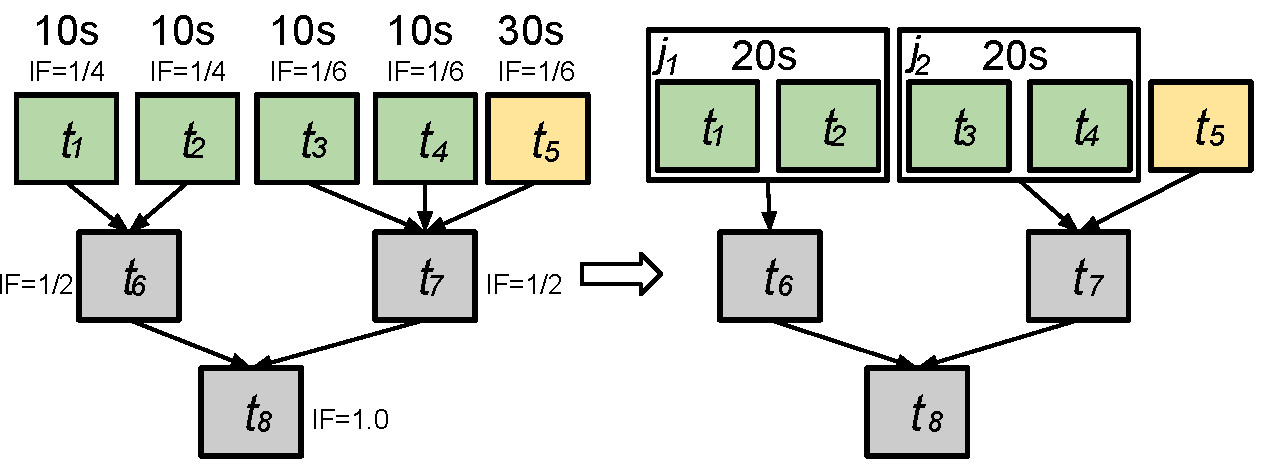
\includegraphics[width=0.75\linewidth]{figures/balance/figure9.pdf}
	\captionof{figure}{An example of the HIFB (Horizontal Impact Factor Balancing) method. Impact factors allow the detection of similarities between tasks.}
	\label{fig:imbalance_hifb}
\end{figure}

However, HIFB is suitable for workflows with asymmetric structure. A symmetric workflow structure means there exists a (usually vertical) division of the workflow graph such that one part of the workflow is a mirror of the other part. For symmetric workflows, such as the one shown in Figure~\ref{fig:imbalance_hrb}, the $IF$ value for all tasks of the first level will be the same ($IF=0.25$), thus the method may also cause dependency imbalance. In HDB, jobs are sorted based on the distance between them and the targeted task $t$, then on their runtimes. 
Algorithm~\ref{alg:imbalance_hdb} shows the pseudocode of HDB. 
For instance, in Figure~\ref{fig:imbalance_hdb}, the distances between tasks $D(t_1,t_2)=D(t_3,t_4)=2$, while $D(t_1,t_3)=D(t_1,t_4)=D(t_2,t_3)=D(t_2,t_4)=4$. Thus, HDB merges a list of candidate tasks with the minimal distance ($t_1$ and $t_2$, and $t_3$ and $t_4$). Note that even if the workflow is asymmetric (Figure~\ref{fig:imbalance_hifb}), HDB would obtain the same result as with HIFB. 

\begin{figure}[!htb]
	\centering
	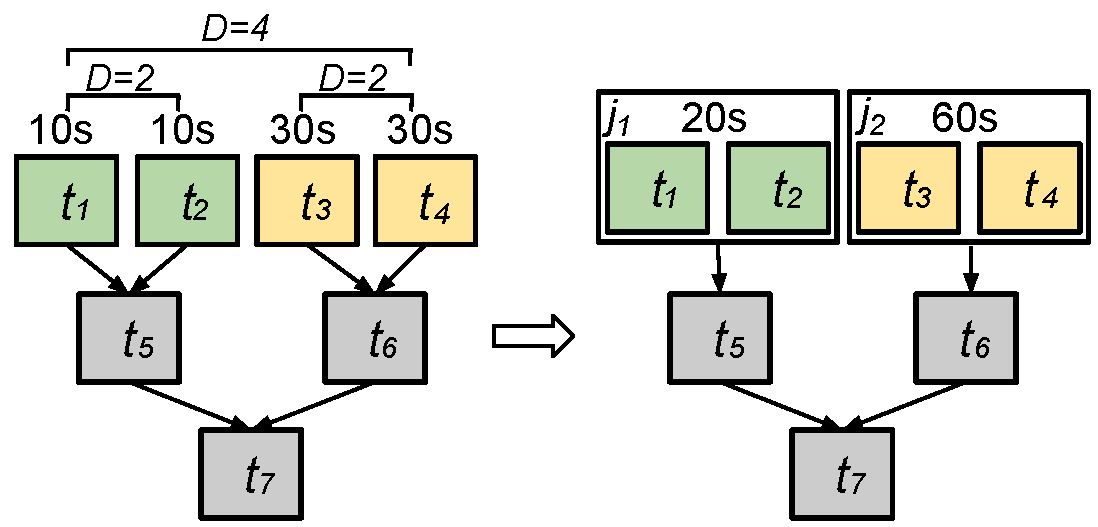
\includegraphics[width=0.7\linewidth]{figures/balance/figure10.pdf}
	\captionof{figure}{An example of the HDB (Horizontal Distance Balancing) method. Measuring the distances between tasks avoids data locality problems.}
	\label{fig:imbalance_hdb}
\end{figure}

There are cases where HDB would yield lower performance than HIFB. For instance, let $t_1$, $t_2$, $t_3$, $t_4$, and $t_5$ be the set of tasks to be merged in the workflow presented in Figure~\ref{fig:imbalance_hifb_hdb}. HDB does not identify the difference in the number of parent/child tasks between the tasks, since $d(t_u,t_v) = 2, \forall u,v \in [1,5], u \neq v$. On the other hand, HIFB does distinguish them since their impact factors are slightly different. Example of such scientific workflows include the LIGO Inspiral workflow~\cite{LIGO}, which is used in the evaluation of this chapter (Section~\ref{sec:balance:results}).

\begin{figure}[!htb]
	\centering
	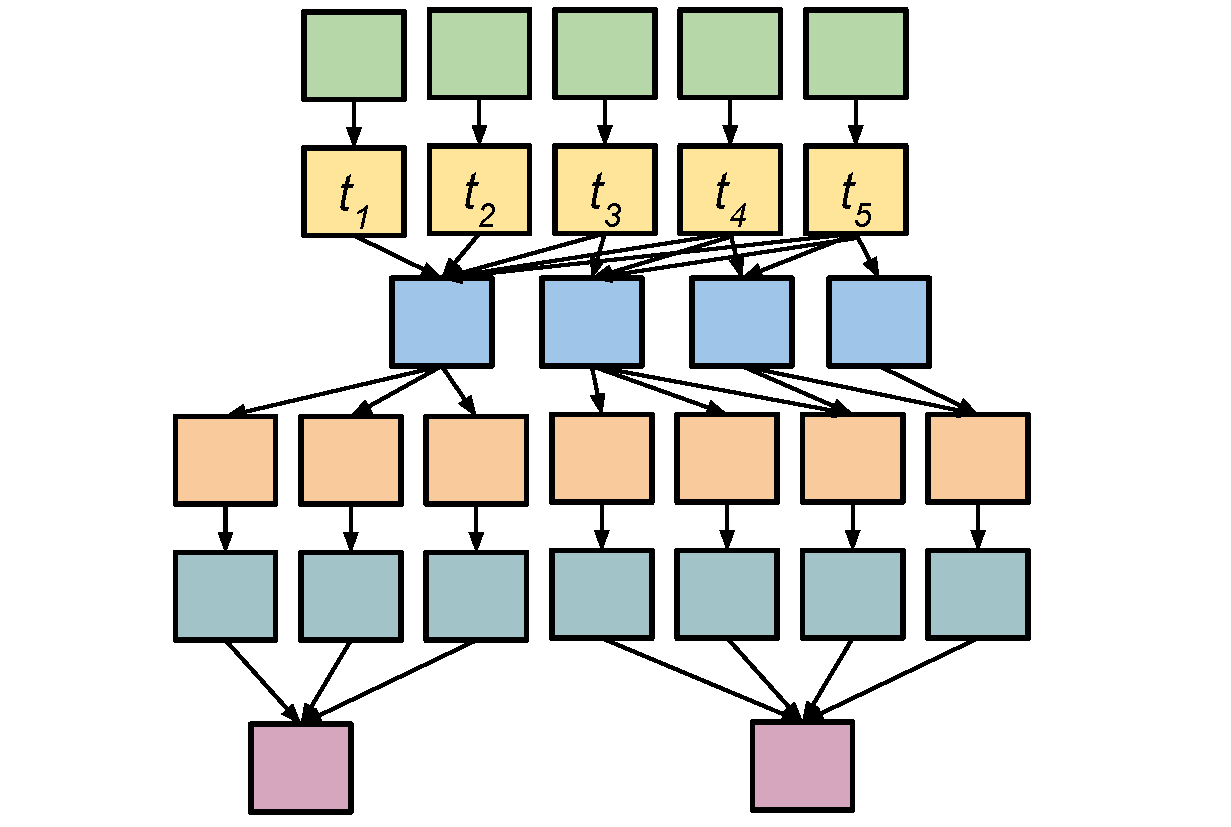
\includegraphics[width=0.75\linewidth]{figures/balance/figure11.pdf}
	\captionof{figure}{A workflow example where HDB yields lower performance than HIFB. HDB does not capture the difference in the number of parents/child tasks, since the distances between tasks ($t_1$, $t_2$, $t_3$, $t_4$, and $t_5$) are the same.}
	\label{fig:imbalance_hifb_hdb}
\end{figure}

Table~\ref{tab:2} summarizes the imbalance metrics and balancing methods presented in this chapter. 

\begin{figure}[htb]
	\centering
	\small
	\begin{tabular}{l|l}
		\hline
		\textbf{Imbalance Metrics} & $abbr.$   \\
		\hline
		Horizontal Runtime Variance & \emph{HRV}   \\ 
%		%Pipeline Runtime Variance &{\em PRV}  \\ 
		Horizontal Impact Factor Variance & \emph{HIFV} \\ 
		Horizontal Distance Variance & \emph{HDV}  \\ 
		\hline
		\textbf{Balancing Methods} & $abbr.$  \\
		\hline
%		Horizontal Clustering & HC \\
		Horizontal Runtime Balancing & HRB   \\ 
%		Vertical Clustering & VC \\ 
		Horizontal Impact Factor Balancing & HIFB\\ 
		Horizontal Distance Balancing & HDB \\ 
		\hline
	\end{tabular}
	\captionof{table}{Summary of imbalance metrics and balancing methods.}
	\label{tab:2}
\end{figure}



\subsection{Combining vertical clustering methods}

In this subsection, we discuss how we combine the balanced clustering methods presented above with vertical clustering (VC).
In pipelined workflows (single-parent-single-child tasks), vertical clustering always yields improvement over a baseline, non-clustered execution because merging reduces system overheads and data transfers within the pipeline. Horizontal clustering does not have the same guarantee since its performance depends on the comparison of system overheads and task durations. However, vertical clustering has limited performance improvement if the workflow does not have pipelines. Therefore, we are interested in the analysis of the performance impact of applying both vertical and horizontal clustering in the same workflow. We combine these methods in two ways: (\emph{i}) \emph{VC-prior}, and (\emph{ii}) \emph{VC-posterior}.


\paragraph{\textbf{VC-prior}}
In this method, vertical clustering is performed first, and then the balancing methods (HRB, HIFB, HDB, or HC) are applied. Figure~\ref{fig:imbalance_vc_prior} shows an example where pipelined-tasks are merged first, and then the merged pipelines are horizontally clustered based on the runtime variance.

\begin{figure}[!htb]
	\centering
	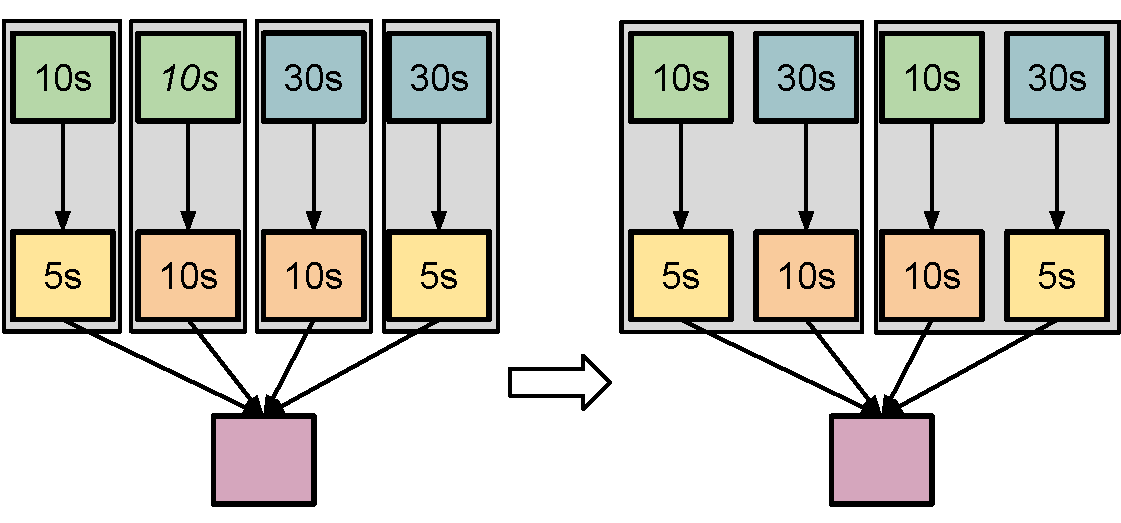
\includegraphics[width=0.75\linewidth]{figures/balance/figure12.pdf}
	\captionof{figure}{\emph{VC-prior}: vertical clustering is performed first, and then the balancing methods.}
	\label{fig:imbalance_vc_prior}
\end{figure}

\paragraph{\textbf{VC-posterior}} 
%Here, vertical clustering is performed \emph{a posteriori}, i.e. balancing methods are first applied, and then VC. Figure~\ref{fig:imbalance_vc_posterior} shows an example where tasks are horizontally clustered first based on the runtime variance, and then merged vertically. In this example, vertical clustering targeted the data locality problem by merging tasks that would not generate interdependency once clustered. However, this approach causes a runtime imbalance problem.

\begin{figure}[!htb]
	\centering
	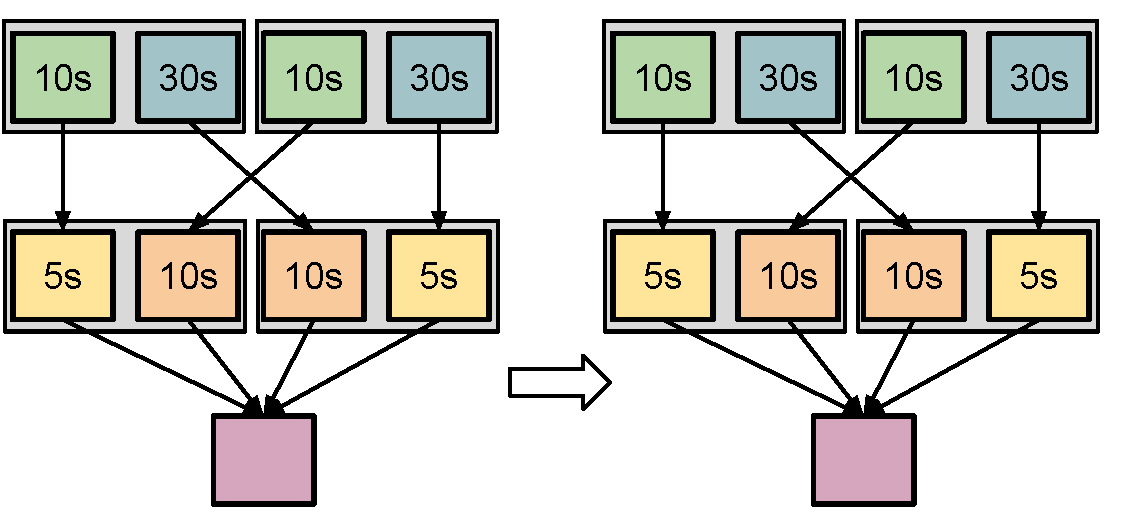
\includegraphics[width=0.75\linewidth]{figures/balance/figure13.pdf}
	\captionof{figure}{\emph{VC-posterior}: horizontal clustering (balancing methods) is performed first, and then vertical clustering (but without changes).}
	\label{fig:imbalance_vc_posterior}
\end{figure}

Here, balancing methods are first applied, and then vertical clustering. Figure~\ref{fig:imbalance_vc_posterior} shows an example where tasks are horizontally clustered first based on the runtime variance, and then merged vertically. However, since the original pipeline structures have been broken by horizontal clustering, VC does not perform any changes to the workflow. 


%means we perform horizontal clustering methods first and then vertical clustering. For the same workflow, assuming we merge tasks horizontally as shown in , we can see that we cannot perform vertical clustering to clustered jobs at the fourth level and the fifth level since the original pipeline structures have been destroyed by horizontal clustering. This phenomenon suggests us VC-posterior may work better compared to VC-prior, generally speaking. However, some opposite cases do exist. We will verify our hypothesis in Section~\ref{sec:results}. We will also compared the two combining approaches with \textbf{VC-only}, which means we perform vertical clustering only and \textbf{No-VC}, which means we just perform horizontal clustering methods without vertical clustering. 








% Section
\section{Evaluation}
\label{sec:balance:experiments}

The experiments presented hereafter evaluate the performance of our balancing methods when compared to an existing and effective task clustering strategy named Horizontal Clustering (HC)~\cite{Singh2008}, which is widely used by workflow management systems such as Pegasus~\cite{Deelman2004}. We also compare our methods with two heuristics described in literature: DFJS~\cite{Muthuvelu2005}, and AFJS~\cite{Liu2009}. DFJS groups bags of tasks based on the task durations up to the resource capacity. AFJS is an extended version of DFJS that is an adaptive fine-grained job scheduling algorithm to group fine-grained tasks according to processing capacity of the current available resources and bandwidth between these resources.

% Task clustering techniques
\subsection{Task clustering techniques}

In the experiments, we compare the performance of our balancing methods to the Horizontal Clustering (HC)~\cite{Singh2008} technique, and with two methods well known from the literature, DFJS~\cite{Muthuvelu2005} and AFJS~\cite{Liu2009}. In this subsection, we briefly describe each of these algorithms.


\paragraph{\textbf{HC}}
Horizontal Clustering (HC) merges multiple tasks that are at the same horizontal level of the workflow. The clustering granularity (number of tasks within a cluster) of a clustered job is controlled by the user, who defines either the number of tasks per clustered job (\emph{clusters.size}), or the number of clustered jobs per horizontal level of the workflow (\emph{clusters.num}). This algorithm has been implemented and used in Pegasus~\cite{Singh2008}. For simplicity, we define \emph{clusters.num} as the number of available resources. In our prior work~\cite{Chen2013b}, we have compared the runtime performance with different clustering granularity. The pseudocode of the HC technique is shown in Algorithm~\ref{alg:balance:evaluation_hc}. 


\begin{algorithm}[!htb]
	\footnotesize
	\caption{Horizontal Clustering algorithm.}
	\label{alg:balance:evaluation_hc}
	\begin{algorithmic}[1]
		\Require $W$: workflow; $C$: max number of tasks per job defined by \emph{clusters.size} or \emph{clusters.num}
		\Procedure{Clustering}{$W,C$}
			\For{$level < depth(W)$}
				\State $TL\gets $\ \Call{GetTasksAtLevel}{$W,level$} \Comment{Partition $W$ based on depth}
				\State $CL\gets$  \ \Call{Merge}{$TL,C$} \Comment{Returns a list of clustered jobs}
				\State $W \gets W - TL + CL$  \Comment{Merge dependencies as well} 
			\EndFor
		\EndProcedure
		\Procedure{Merge}{$TL, C$}
			\State $J\gets$ \{\}\Comment{An empty job}
			\State $CL\gets$\{\}\Comment{An empty list of clustered jobs}
			\While{$TL$ is not empty}
				\State $J$.add ($TL$.pop($C$) \Comment{Pops $C$ tasks that are not merged }
				\State  $CL$.add( $J$)
			\EndWhile
			\State \textbf{return} $CL$
		\EndProcedure
	\end{algorithmic}
\end{algorithm}

\paragraph{\textbf{DFJS}}
The dynamic fine-grained job scheduler (DFJS) was proposed by Muthuvelu et al.~\cite{Muthuvelu2005}. The algorithm groups bags of tasks based on their granularity size---defined as the processing time of the task on the resource. Resources are ordered by their decreasing values of capacity (in MIPS), and tasks are grouped up to the resource capacity. This process continues until all tasks are grouped and assigned to resources. Algorithm~\ref{alg:evaluation_dfjs} shows the pseudocode of the heuristic. 
 
\begin{algorithm}[!htb]
	\caption{ DFJS algorithm.}
	\footnotesize
	\label{alg:evaluation_dfjs}
	\begin{algorithmic}[1]
		\Require $W$: workflow; $max.runtime$: max runtime of clustered jobs 
		\Procedure{Clustering}{$W,max.runtime$}
			\For{$level < $the depth of $W$}
				\State $TL\gets $\ \Call{GetTasksAtLevel}{$W,level$} \Comment{Partition $W$ based on depth}
				\State $CL\gets$  \ \Call{Merge}{$TL,max.runtime$} \Comment{Returns a list of clustered jobs}
				\State $W \gets W - TL + CL$  \Comment{Merge dependencies as well} 
			\EndFor
		\EndProcedure
		\Procedure{Merge}{$TL, max.runtime$}
			\State $J\gets$ \{\}\Comment{An empty job}
			\State $CL\gets$\{\}\Comment{An empty list of clustered jobs}
			\While{$TL$ is not empty}
				\State $t \gets TC$.pop() \Comment{Get a task that is not mereged}
				\If {$J$.runtime + $t$.runtime $> max.runtime$}
				\State	$CL$.add($J$)
				\State	$J \gets$\{\}
				\EndIf	
				\State $J$.add($t$)
			\EndWhile
			\State \textbf{return} $CL$
		\EndProcedure
	\end{algorithmic}
\end{algorithm}


\paragraph{\textbf{AFJS}}
The adaptive fine-grained job scheduler (AFJS)~\cite{Liu2009} is an extension of DFJS. It groups tasks not only based on the maximum runtime defined per cluster job, but also on the maximum data size per clustered job. The algorithm adds tasks to a clustered job until the job's runtime is greater than the maximum runtime or the job's total data size (input + output) is greater than the maximum data size. The AFJS heuristic pseudocode is shown in Algorithm~\ref{alg:evaluation_afjs}. 

\begin{algorithm}[!htb]
	\caption{ AFJS algorithm.}
	\footnotesize
	\label{alg:evaluation_afjs}
	\begin{algorithmic}[1]
		\Require $W$: workflow; $max.runtime$: the maximum runtime for a clustered jobs; $max.datasize$: the maximum data size for a clustered job
		\Procedure{Clustering}{$W,max.runtime$}
			\For{$level < $the depth of $W$}
				\State $TL\gets $\ \Call{GetTasksAtLevel}{$W,level$} \Comment{Partition $W$ based on depth}
				\State $CL\gets$  \ \Call{Merge}{$TL,max.runtime, max.datasize$} \Comment{Returns a list of clustered jobs}
				\State $W \gets W - TL + CL$  \Comment{Merge dependencies as well} 
			\EndFor
		\EndProcedure
		\Procedure{Merge}{$TL, max.runtime, max.datasize$}
			\State $J\gets$ \{\}\Comment{An empty job}
			\State $CL\gets$\{\}\Comment{An empty list of clustered jobs}
			\While{$TL$ is not empty}
				\State $t \gets TC$.pop() \Comment{Get a task that is not mereged}
				\If {$J$.runtime + $t$.runtime $> max.runtime$ OR $J$.datasize + $t$.datasize $> max.datasize$}
				\State	$CL$.add($J$)
				\State	$J \gets$\{\}
				\EndIf	
				\State $J$.add($t$)
			\EndWhile
			\State \textbf{return} $CL$
		\EndProcedure
	\end{algorithmic}
\end{algorithm}

DFJS and AFJS require parameter tuning (e.g. maximum runtime per clustered job) to efficiently cluster tasks into coarse-grained jobs. For instance, if the maximum runtime is too high, all tasks may be grouped into a single job, leading to loss of parallelism. In contrast, if the runtime threshold is too low, the algorithms do not group tasks, leading to no improvement over a baseline execution. 

For comparison purposes, we perform a parameter study in order to tune the algorithms for each workflow application described in Section~\ref{sec:applications}. Exploring all possible parameter combinations is a cumbersome and exhaustive task. In the original DFJS and AFJS works, these parameters are empirically chosen, however this approach requires deep knowledge about the workflow applications. Instead, we performed a parameter tuning study, where we first estimate the upper bound of \emph{max.runtime} ($n$) as the sum of all task runtimes, and the lower bound of \emph{max.runtime} ($m$) as 1 second for simplicity. Data points are divided into ten chunks and then we sample one data point from each chunk. We then select the chunk that has the lowest makespan and set $n$ and $m$ as the upper and lower bounds of the selected chunk, respectively. These steps are repeated until $n$ and $m$ have converged into a data point.

%We do not provide a mathematical proof of the correctness of our method, since we are not focused on demonstrating the optimal tuning for DFJS and AFJS algorithms, but a rough estimation of the minimal makespan. Instead, 

To demonstrate the correctness of our sampling approach in practice, we show the relationship between the makespan and the \emph{max.runtime} for an example Montage workflow application in Figure~\ref{fig:evaluation_dfjs_montage}---experiment conditions are presented in Section~\ref{sec:balance:experiment_conditions}. Data points are divided into 10 chunks of 250s each (for \emph{max.runtime}). As the lower makespan values belongs to the first chunk, $n$ is updated to 250, and $m$ to 1. The process repeats until the convergence around \emph{max.runtime}=180s. Even though there are multiple local minimal makespan values, these data points are close to each other, and the difference between their values (on the order of seconds) is small enough to be ignored.

\begin{figure}[!htb]
	\centering
	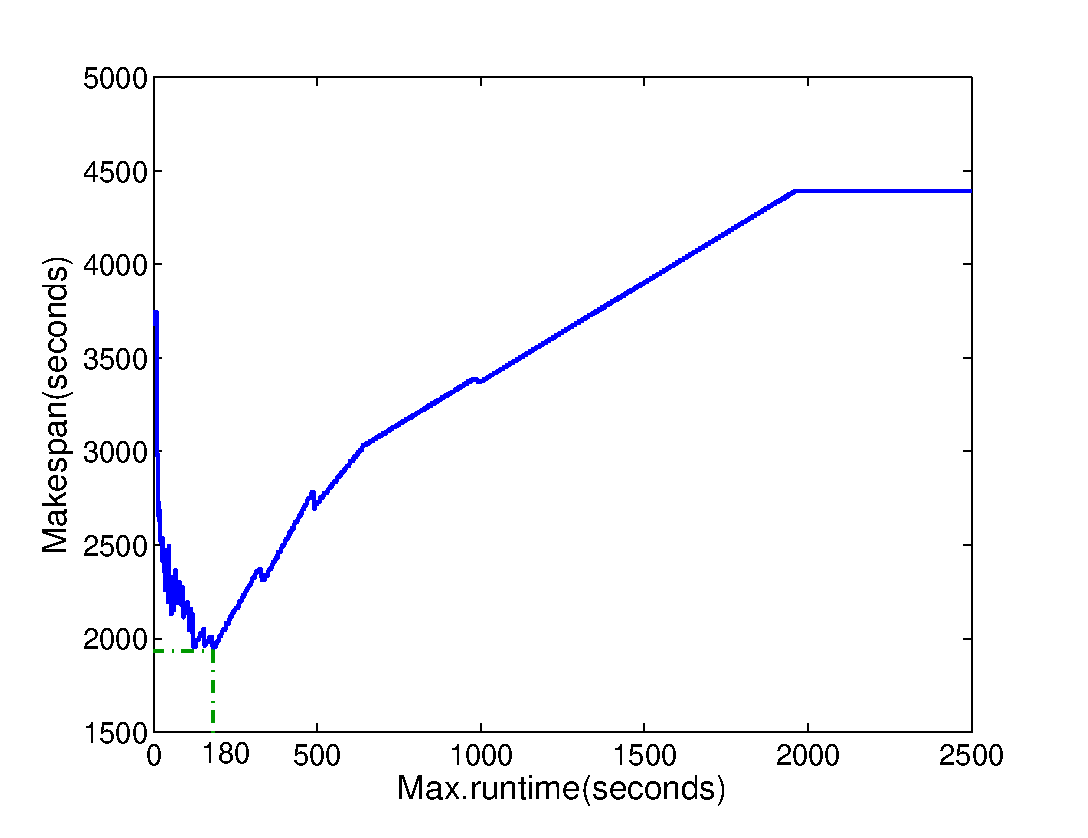
\includegraphics[width=.6\linewidth]{figures/balance/figure19.eps}
	\captionof{figure}{Relationship between the makespan of workflow and the specified maximum runtime in DFJS (Montage).}
	\label{fig:evaluation_dfjs_montage}
\end{figure}

For simplicity, in the rest of this chapter we use DFJS* and AFJS* to indicate the best estimated performance of DFJS and AFJS respectively using the sampling approach described above.


% Experiment conditions
\subsection{Experiment conditions}
\label{sec:balance:experiment_conditions}
We adopt a trace-based simulation approach, where we extended our WorkflowSim~\cite{WorkflowSim} simulator with the balanced clustering methods and imbalance metrics to simulate a controlled distributed environment. 
The simulated computing platform is composed by 20 single homogeneous core virtual machines (worker nodes), which is the quota per user of some typical distributed environments such as Amazon EC2~\cite{AmazonAWS} and FutureGrid~\cite{Fox2013FutureGrid}. Each simulated virtual machine (VM) has 512MB of memory and the capacity to process 1,000 million instructions per second. The default network bandwidth is 15MB according to the real environment in FutureGrid from where our traces were collected. The task scheduling algorithm is data-aware, i.e. tasks are scheduled to resources which have the most input data available. By default, we merge tasks at the same horizontal level into 20 clustered jobs, which is a simple selection of granularity control of the strength of task clustering. The study of granularity size has been done in~\cite{Chen2013b}, which shows such selection is acceptable. 

We collected workflow execution traces~\cite{Juve2013,Chen2011} (including overhead and task runtime information) from real runs (executed on FutureGrid and Amazon EC2) of the scientific workflow applications described in Section~\ref{sec:applications}. The traces are used to feed the Workflow Generator toolkit~\cite{WorkflowGenerator} to generate synthetic workflows. This allows us to perform simulations with different configurations under controlled conditions. The toolkit uses the information gathered from actual scientific workflow executions to generate synthetic workflows resembling those used by real world scientific applications. The number of inputs to be processed, the number of tasks in the workflow, and their composition determine the structure of the generated workflow. Such an approach of traced based simulation allows us to utilize real traces and vary the system setting (i.e., the number of VMs) and workflow (i.e., avg. data size) to fully explore the performance of our balancing algorithms. 

Three sets of experiments are conducted. Experiment 1 evaluates the performance gain ($\mu$) of our balancing methods (HRB, HIFB, and HDB) over a baseline execution that has no task clustering. We define the performance gain over a baseline execution ($\mu$) as the performance of the balancing methods related to the performance of an execution without clustering. Thus, for values of $\mu > 0$ our balancing methods perform better than the baseline execution. Otherwise, the balancing methods perform poorer. The goal of the experiment is to identify conditions where each method works best and worst. In addition, we also evaluate the performance gain of using workflow structure metrics (HRV, HIFV, and HDV), which require fewer \emph{a-priori} knowledge from task and resource characteristics, over task clustering techniques in literature (HC, DFJS*, and AFJS*).

Experiment 2 evaluates the performance impact of the variation of average data size (defined as the average of all the input and output data) and the number of resources available in our balancing methods for one scientific workflow application (LIGO). The original average data size (both input and output data) of the LIGO workflow is about 5MB as shown in Table~\ref{tab:model_workflows}. In this experiment, we increase the average data size up to 500MB to study the behavior of data-intensive workflows. We control resource contention by varying the number of available resources (VMs). High resource contention is achieved by setting the number of available VMs to 5, which represents less than 10\% of the required resources to compute all tasks in parallel. On the other hand, low contention is achieved when the number of available VMs is increased to 25, which represents about 50\% of the required resources.

Experiment 3 evaluates the influence of combining our horizontal clustering methods with vertical clustering (VC). We compare the performance gain under four scenarios: (\emph{i}) \emph{VC-prior}, VC is first performed and then HRB, HIFB, or HDB; (\emph{ii}) \emph{VC-posterior}, horizontal methods are performed first and then VC; (\emph{iii}) \emph{No-VC}, horizontal methods only; and (\emph{iv}) \emph{VC-only}, no horizontal methods. Table~\ref{tab:evaluation_vc_combination} shows the results of combining VC with horizontal methods. For example, VC-HIFB indicates we perform VC first and then HIFB. 
%The motivation behind this experiment is that we believe VC will change imbalance metrics (HIFV, HDV and HRV) and we aim to show how these metrics can help us understand the performance of VC better. 

\begin{table}[!htb]
	%\setlength{\tabcolsep}{11pt}
	\centering
	\small
	\begin{tabular}{l|rrrr}
		\hline
		Combination	& HIFB	 &  HDB & HRB & HC \\
		\hline
		VC-prior 		& VC-HIFB		& VC-HDB	& VC-HRB & VC-HC\\
		VC-posterior 		&HIFB-VC		&HDB-VC	&HRB-VC & HC-VC\\
		VC-only 	&VC		&VC 	& VC & VC\\
		No-VC 	&HIFB 	& HDB & HRB	& HC \\
		\hline
	\end{tabular}
	\caption{Combination Results. `-' indidates the order of performing these algorithms, i.e., VC-HIFB indicates we perform VC first and then HIFB}
	\label{tab:evaluation_vc_combination}
\end{table} 




% Results and discussion
\subsection{Results and discussion}
\label{sec:balance:results}
\paragraph{\textbf{Experiment 1}}
Figure~\ref{fig:evaluation_algorithm} shows the performance gain $\mu$ of the balancing methods for the five workflow applications over a baseline execution. All clustering techniques significantly improve (up to 48\%) the runtime performance of all workflow applications, except HC for SIPHT. The reason is that SIPHT has a high HRV compared to other workflows as shown in Table~\ref{tab:evaluation_montage}. This indicates that the runtime imbalance problem in SIPHT is more significant and thus it is harder for HC to achieve performance improvement. Cybershake and Montage workflows have the highest gain but nearly the same performance independent of the algorithm. This is due to their symmetric structure and low values for the imbalance metrics and the distance metrics as shown in Table~\ref{tab:evaluation_montage}. 
Epigenomics and LIGO have higher average task runtime and thus the lower performance gain. However, Epigenomices and LIGO have higher variance of runtime and distance and thus the performance improvement of HRB and HDB is better than that of HC, which is more significant compared to other workflows. 
In particular, each branch of the Epigenomics workflow (Figure~\ref{fig:model_shape_genome}) has the same number of pipelines, consequently the $IF$ values of tasks in the same horizontal level are the same. Therefore, HIFB cannot distinguish tasks from different branches, which leads the system to a dependency imbalance problem. In such cases, HDB captures the dependency between tasks and yields better performance. Furthermore, Epigenomics and LIGO workflows have high runtime variance, which has higher impact on the performance than data dependency. Last, the performance gain of our balancing methods is better than the tuned algorithms DFJS* and AFJS* in most cases. The other benefit is that our balancing methods do not require parameter tuning, which is cumbersome in practice. 

\begin{figure}[htb]
	\centering
	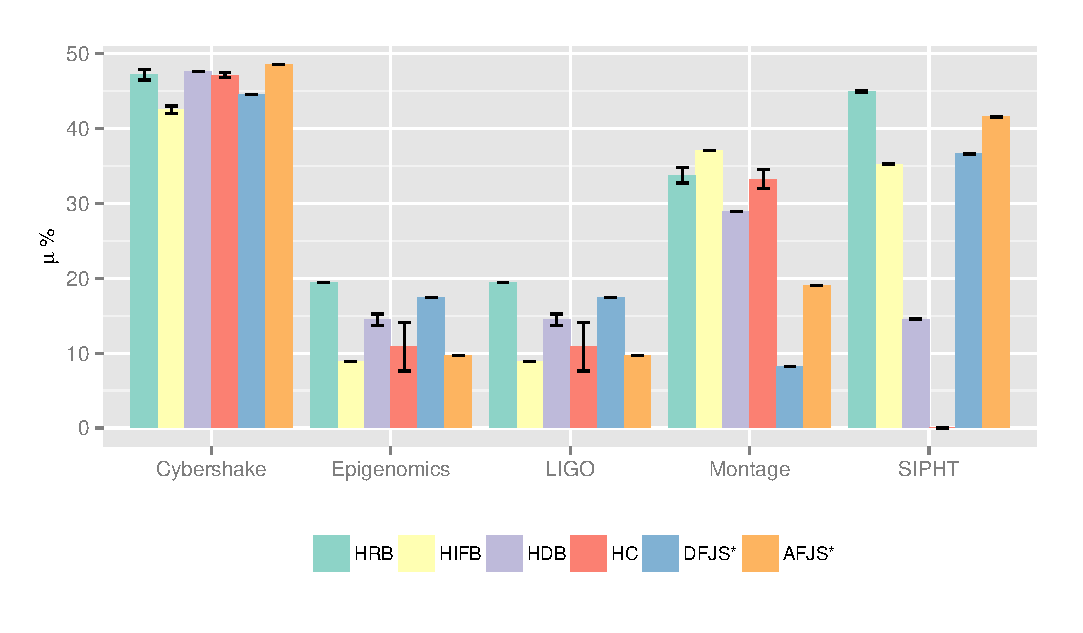
\includegraphics[width=0.8\linewidth]{figures/balance/figure20.eps}
	\captionof{figure}{Experiment 1: performance gain ($\mu$) over a baseline execution for six algorithms (*~indicates the tuned performance of DFJS and AFJS). By default, we have 20 VMs. }
	\label{fig:evaluation_algorithm}
\end{figure}

\begin{table}[!htb]
	\setlength{\tabcolsep}{12pt}
	\centering
	\small
	\begin{tabular}{c|r|r|r|r}
		& \# of Tasks & HRV &  HIFV & HDV  \\ \hline
		Level & \multicolumn{4}{c}{(a) \textbf{CyberShake}} \\
		\hline
		1 & 4 & 0.309 & 0.03 & 1.22 \\
		2 & 347 & 0.282 & 0.00 & 0.00 \\
		3 & 348 & 0.397 & 0.00 & 26.20 \\
		4 & 1 & 0.000 & 0.00 & 0.00 \\
		\hline
		Level & \multicolumn{4}{c}{(b) \textbf{Epigenomics}} \\
		\hline
		1 & 3 & 0.327 & 0.00 & 0.00  \\
		2 & 39 & 0.393 & 0.00 & 578 \\
		3 & 39 & 0.328 & 0.00 & 421 \\
		4 & 39 & 0.358 & 0.00 & 264 \\
		5 &39 & 0.290 & 0.00 & 107 \\
		6 & 3 & 0.247 & 0.00 & 0.00  \\
		7 &1  & 0.000 & 0.00 & 0.00 \\
		8 &1 & 0.000 & 0.00 & 0.00 \\
		9 & 1 & 0.000 & 0.00 & 0.00 \\
		\hline
		Level & \multicolumn{4}{c}{(c) \textbf{LIGO}} \\
		\hline
		1 & 191 & 0.024 & 0.01 & 10097 \\
		2 & 191 & 0.279 & 0.01 & 8264 \\
		3 & 18 & 0.054 & 0.00 & 174 \\
		4 & 191 & 0.066 & 0.01 & 5138 \\
		5 & 191 & 0.271 & 0.01 & 3306 \\
		6 & 18 &  0.040 & 0.00 & 43.70 \\
		\hline		
		Level & \multicolumn{4}{c}{(d) \textbf{Montage}} \\
		\hline
		1 &49 & 0.022 & 0.01 & 189.17 \\
		2 & 196 & 0.010 & 0.00 & 0.00 \\
		3 & 1 & 0.000 & 0.00 & 0.00 \\
		4 & 1 & 0.000 & 0.00 & 0.00 \\
		5 &49 & 0.017 & 0.00 & 0.00 \\
		6 & 1 & 0.000 & 0.00 & 0.00 \\
		7 &1  & 0.000 & 0.00 & 0.00 \\
		8 &1 & 0.000 & 0.00 & 0.00 \\
		9 & 1 & 0.000 & 0.00 & 0.00 \\
		\hline		
		Level & \multicolumn{4}{c}{(e) \textbf{SIPHT}} \\
		\hline
		1 & 712 & 3.356 & 0.01 & 53199 \\
		2 & 64 & 1.078 & 0.01 & 1196 \\
		3 & 128 & 1.719 & 0.00 & 3013 \\
		4 & 32 & 0.000 & 0.00 & 342 \\
		5 & 32 & 0.210 & 0.00 & 228\\
		6& 32 & 0.000 & 0.00 & 114\\
	\end{tabular}
	\caption{Experiment 1: average number of tasks, and average values of imbalance metrics (HRV, HIFV, and HDV) for the 5 workflow applications (before task clustering).}
	\label{tab:evaluation_montage}
\end{table} 


\paragraph{\textbf{Experiment 2}} 
Figure~\ref{fig:evaluation_datasize} shows the performance gain $\mu$ of HRB, HIFB, HDB, and HC over a baseline execution for the LIGO Inspiral workflow. We chose LIGO because the performance improvement among these balancing methods is significantly different for LIGO compared to other workflows as shown in Figure~\ref{fig:evaluation_algorithm}. For small data sizes (up to 100 MB), the application is CPU-intensive and runtime variations have higher impact on the performance of the application. Thus, HRB performs better than any other balancing method. When increasing the data average size, the application turns into a data-intensive application, i.e. data dependencies have higher impact on the application's performance. HIFB captures both the workflow structure and task runtime information, which reduces data transfers between tasks and consequently yields better performance gain over the baseline execution. HDB captures the strong connections between tasks (data dependencies), while HIFB captures the weak connections (similarity in terms of structure). In some cases, HIFV is zero while HDV is less likely to be zero.
Most of the LIGO branches are like the ones in Figure~\ref{fig:model_shape_ligo}, however, as mentioned in Section~\ref{sec:balance:methods}, the LIGO workflow has a few branches that depend on each other as shown in Figure~\ref{fig:imbalance_hifb_hdb}. Since most branches are isolated from each other, HDB initially performs well compared to HIFB. However, with the increase of average data size, the performance of HDB is more constrained by the interdependent branches, which is shown in Figure~\ref{fig:evaluation_datasize}.  
HC has nearly constant performance despite of the average data size, due to its random merging of tasks at the same horizontal level regardless of the runtime and data dependency information.

\begin{figure}[!htb]
	\centering
    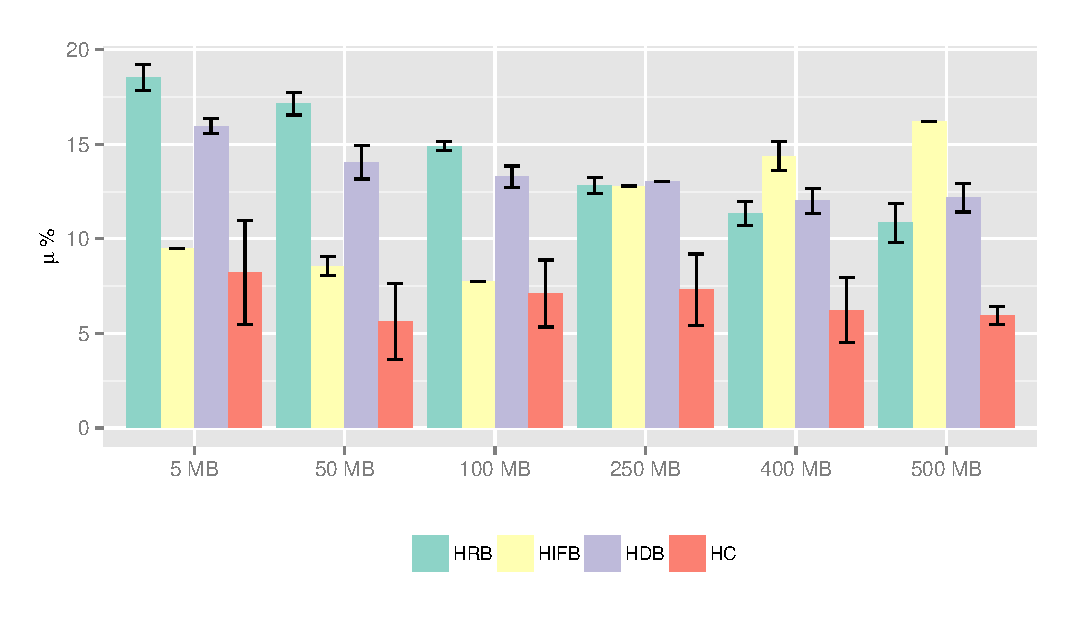
\includegraphics[width=0.8\linewidth]{figures/balance/figure21.eps}
    \caption{Experiment 2: performance gain ($\mu$) over a baseline execution with different average data sizes for the LIGO workflow. The original avg. data size is 5MB.}
    \label{fig:evaluation_datasize}
\end{figure}

Figures~\ref{fig:evaluation_resource_1} and~\ref{fig:evaluation_resource_2} show the performance gain $\mu$ when varying the number of available VMs for the LIGO workflows with an average data size of 5MB (CPU-intensive) and 500MB (data-intensive) respectively. In high contention scenarios (small number of available VMs), all methods perform similar when the application is CPU-intensive (Figure~\ref{fig:evaluation_resource_1}), i.e., runtime variance and data dependency have smaller impact than the system overhead (e.g. queuing time). As the number of available resources increases, and the data size is too small, runtime variance has more impact on the application's performance, thus HRB performs better than the others. Note that as HDB captures strong connections between tasks, it is less sensitive to the runtime variations than HIFB, thus it yields better performance. For the data-intensive case (Figure~\ref{fig:evaluation_resource_2}), data dependencies have more impact on the performance than the runtime variation. In particular, in the high contention scenario HDB performs poor task clustering leading the system to data locality problems compared to HIFB due to the interdependent branches in the LIGO workflow. However, the method still improves the execution due to the high system overhead. Similar to the CPU-intensive case, under low contention, runtime variance increases its importance and then HRB performs better.

\begin{figure}[!htb]
	\centering
	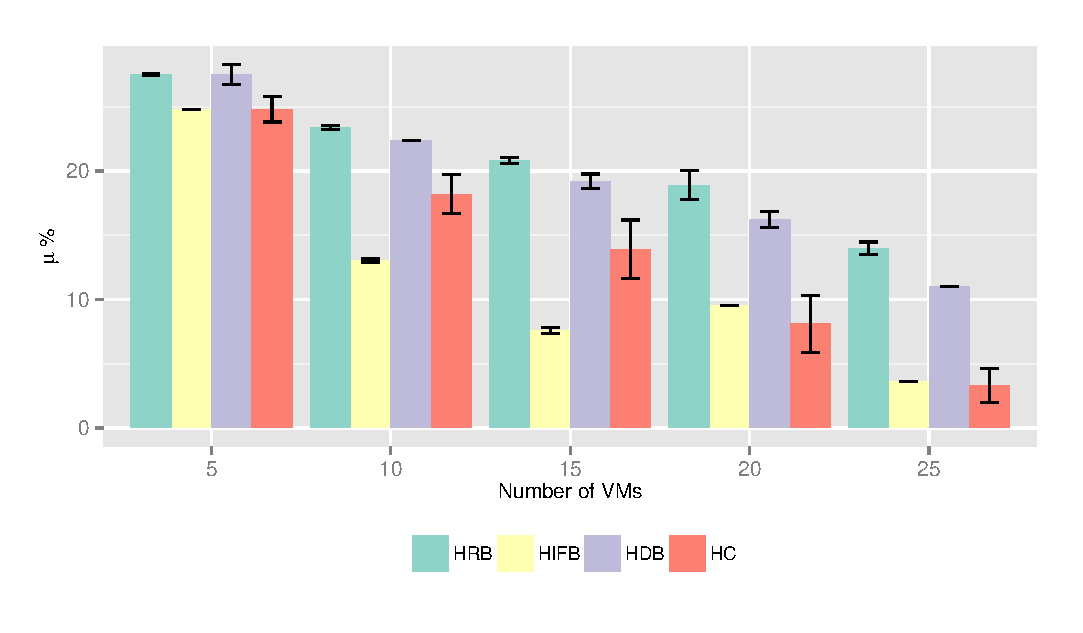
\includegraphics[width=0.8\linewidth]{figures/balance/figure22.eps}
	\captionof{figure}{Experiment 2: performance gain ($\mu$) over baseline execution with different number of resources for the LIGO workflow (average data size is 5MB).}
	\label{fig:evaluation_resource_1}
\end{figure}

\begin{figure}[!htb]
	\centering
	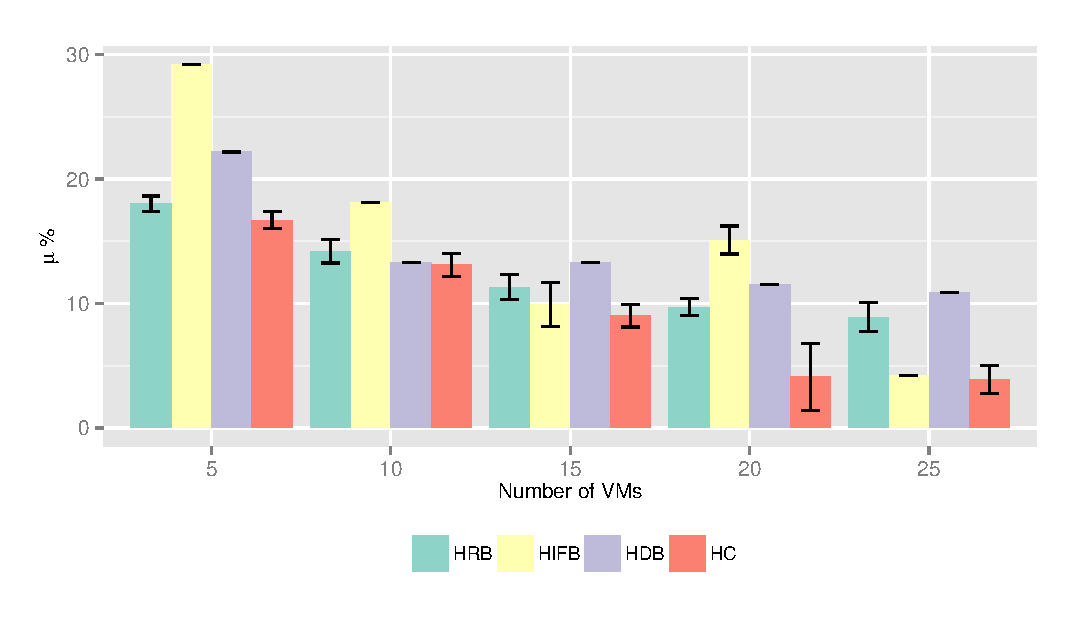
\includegraphics[width=0.8\linewidth]{figures/balance/figure23.eps}
	\captionof{figure}{Experiment 2: performance gain ($\mu$) over baseline execution with different number of resources for the LIGO workflow (average data size is 500MB).}
	\label{fig:evaluation_resource_2}
\end{figure}


\paragraph{\textbf{Experiment 3}}
Figure~\ref{fig:evaluation_vc_cybershake} shows the performance gain $\mu$ for the Cybershake workflow over the baseline execution when using vertical clustering (VC) combined to our balancing methods. Vertical clustering does not aggregate any improvement to the Cybershake workflow ($\mu$(\emph{VC-only}) $\approx 0.2\%$), because the workflow structure has no explicit pipeline (see Figure~\ref{fig:model_shape_cybershake}). Similarly, VC does not improve the SIPHT workflow due to the lack of pipelines on its structure (Figure~\ref{fig:model_shape_sipht}). Thus, results for this workflow are omitted.

\begin{figure}[!htb]
	\centering
	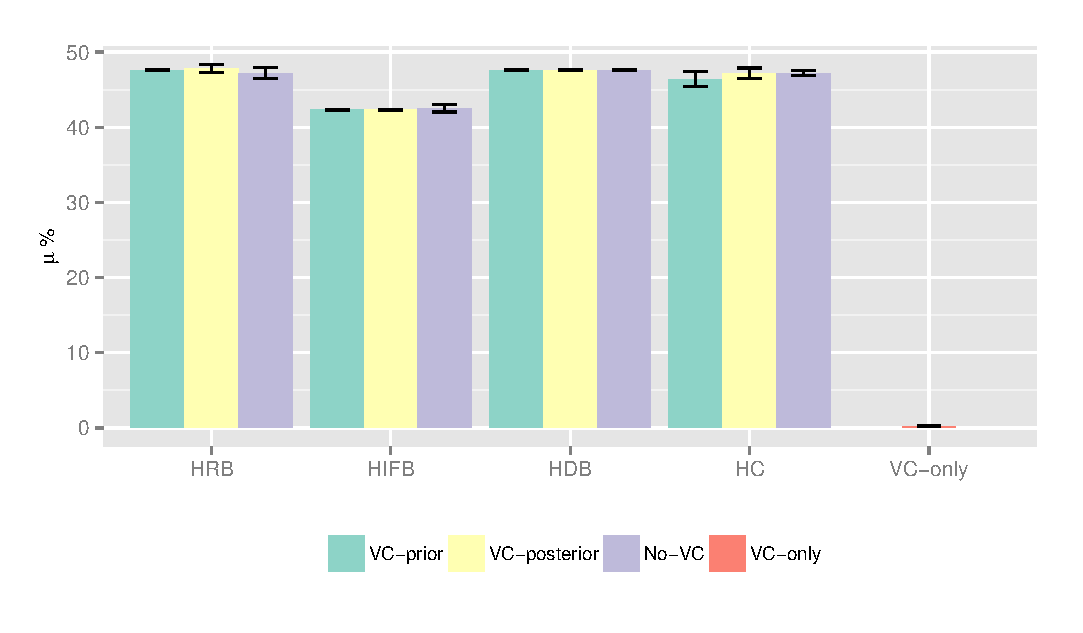
\includegraphics[width=0.8\linewidth]{figures/balance/figure24.eps}
	\captionof{figure}{Experiment 3: performance gain ($\mu$) for the Cybershake workflow over baseline execution when using vertical clustering (VC).}
	\label{fig:evaluation_vc_cybershake}
\end{figure}

Figure~\ref{fig:evaluation_vc_montage} shows the performance gain $\mu$ for the Montage workflow. In this workflow, vertical clustering is often performed on the two pipelines (Figure~\ref{fig:model_shape_montage}). These pipelines are commonly single-task levels, thereby no horizontal clustering is performed on the pipelines. As a result, whether performing vertical clustering prior or after horizontal clustering, the result is about the same. Since VC and horizontal clustering methods are independent with each other in this case, we still should do VC in combination with horizontal clustering to achieve further performance improvement. 

\begin{figure}[!htb]
	\centering
	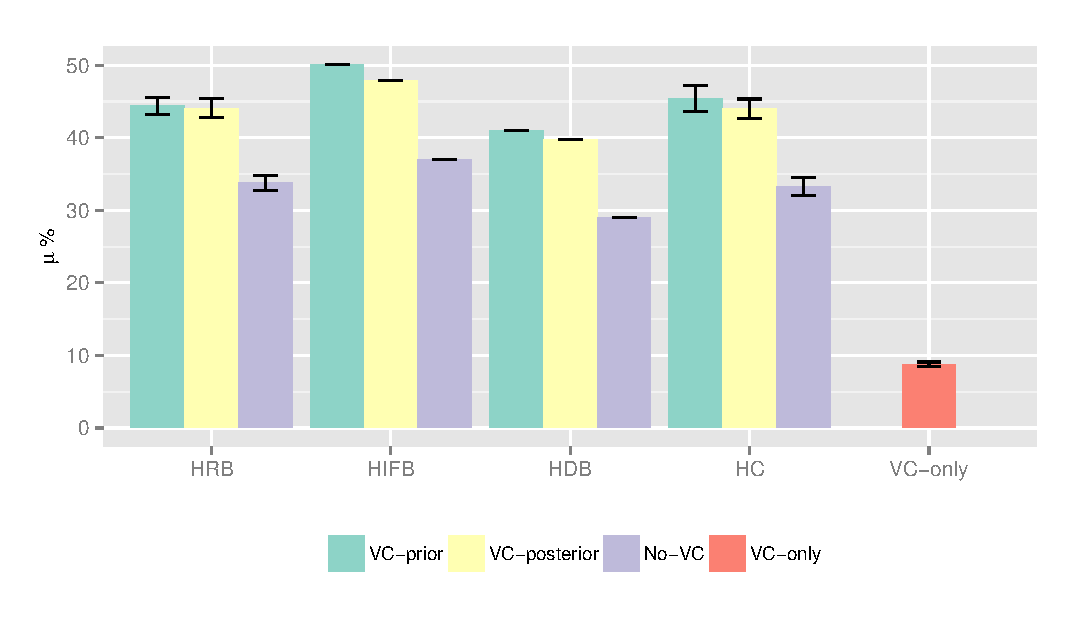
\includegraphics[width=0.8\linewidth]{figures/balance/figure25.eps}
	\captionof{figure}{Experiment 3: performance gain ($\mu$) for the Montage workflow over baseline execution when using vertical clustering (VC).}
	\label{fig:evaluation_vc_montage}
\end{figure}

\begin{figure}[!htb]
	\centering
	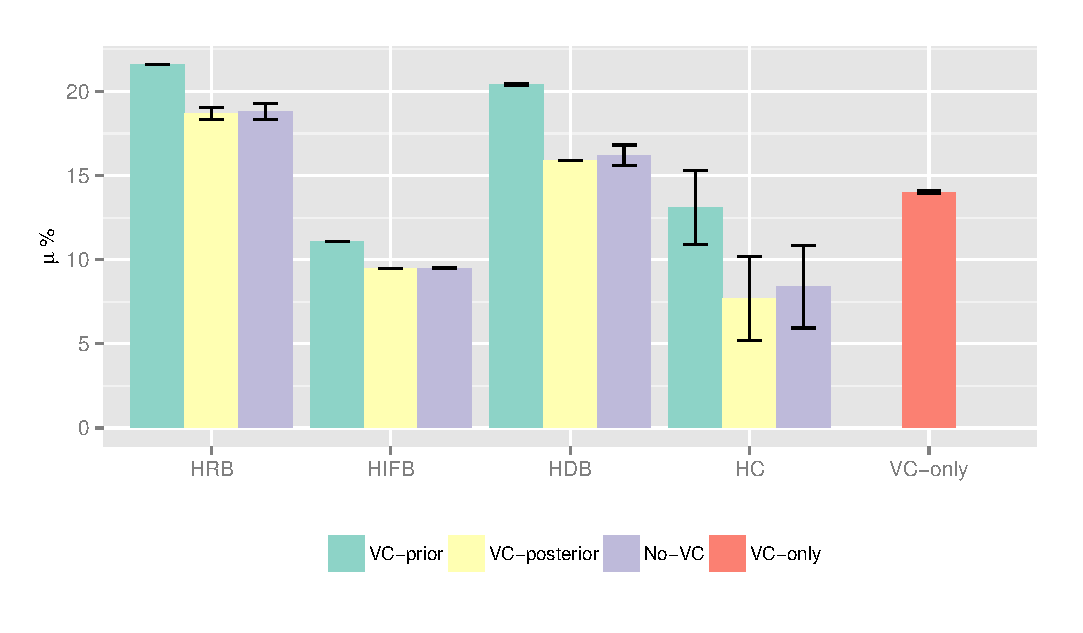
\includegraphics[width=0.8\linewidth]{figures/balance/figure26.eps}
	\captionof{figure}{Experiment 3: performance gain ($\mu$) for the LIGO workflow over baseline execution when using vertical clustering (VC).}
	\label{fig:evaluation_vc_ligo}
\end{figure}


\begin{figure}[!htb]
	\centering
	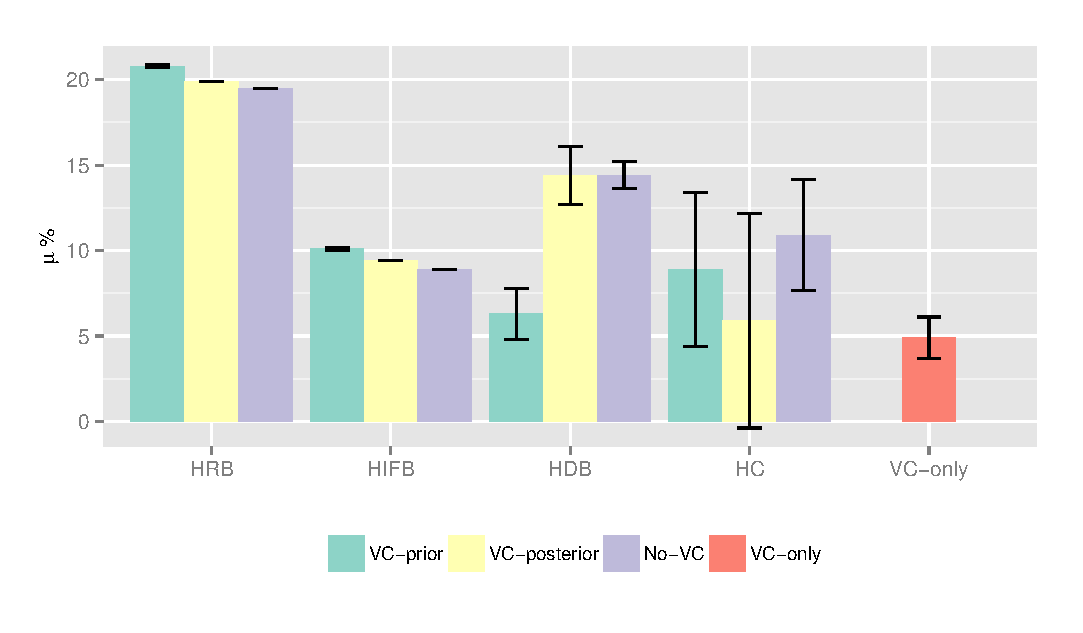
\includegraphics[width=0.8\linewidth]{figures/balance/figure27.eps}
	\captionof{figure}{Experiment 3: performance gain ($\mu$) for the Epigenomics workflow over baseline execution when using vertical clustering (VC).}
	\label{fig:evaluation_vc_genome}
\end{figure}

The performance gain $\mu$ for the LIGO workflow is shown in Figure~\ref{fig:evaluation_vc_ligo}. Vertical clustering yields better performance gain when it is performed prior to horizontal clustering (\emph{VC-prior}). The LIGO workflow structure (Figure~\ref{fig:model_shape_ligo}) has several pipelines that are primarily clustered vertically and thus system overheads (e.g. queuing and scheduling times) are reduced. Furthermore, the runtime variance (HRV) of the clustered pipelines increases, thus the balancing methods, in particular HRB, can further improve the runtime performance by evenly distributing task runtimes among clustered jobs. When vertical clustering is performed \emph{a posteriori}, pipelines are broken due to the horizontally merging of tasks between pipelines neutralizing vertical clustering improvements.





Similarly to the LIGO workflow, the performance gain $\mu$ values for the Epigenomics workflow (see Figure~\ref{fig:evaluation_vc_genome}) are better when VC is performed \emph{a priori}. This is due to several pipelines inherent to the workflow structure (Figure~\ref{fig:model_shape_genome}). However, vertical clustering has poorer performance if it is performed prior to the HDB algorithm. The reason is that the average task runtime of Epigenomics is much larger than other workflows as shown in Table.~\ref{tab:model_workflows}. Therefore, \emph{VC-prior} generates very large clustered jobs vertically and makes it difficult for horizontal methods to improve further. 


In a word, these experiments show strong connections between the imbalance metrics and the performance improvement of the balancing methods we proposed. HRV indicates the potential performance improvement for HRB. The higher HRV is, the more performance improvement HRB is likely to have. Similarly, for symmetric workflows (such as Epigenomics), their HIFV and HDV values are low and thus neither HIFB or HDB performs well. 




\section{Summary}

We presented three balancing methods and two vertical clustering combination approaches to address the load balance problem when clustering workflÇow tasks. We also defiÅned three imbalance metrics to quantitatively measure workflÇow characteristics based on task runtime variation (HRV), task impact factor (HIFV), and task distance variance (HDV).

Three experiment sets were conducted using traces from five real workflow applications. The first experiment aimed at measuring the performance gain over a baseline execution without clustering. In addition, we compared our balancing methods with three algorithms in literature. Experimental results show that our methods yield significant improvement over a baseline execution, and that they have acceptable performance when compared to the best estimated performance of the existing algorithms. The second experiment measured the influence of average data size and number of available resources on the performance gain. In particular, results show that our methods have different sensitivity to data- and computational-intensive workflows. Finally, the last experiment evaluated the interest of performing horizontal and vertical clustering in the same workflow. Results show that vertical clustering can significantly improve pipeline-structured workflows, and it is not suitable if the workflow has no explicit pipelines.

The simulation based evaluation also shows that the performance improvement of the proposed balancing algorithms (HRB, HDB and HIFB) is highly related to the metric values (HRV, HDV and HIFV) that we introduced. For example, a workflow with high HRV tends to have better performance improvement with HRB since HRB is used to balance the runtime variance. 

This chapter has provided a novel approach to address the problem of load imbalance in task clustering. However, the dynamic features of modern distributed systems have brought us new challenges. For example, task clustering strategies in a faulty execution environment may fail to maintain their performance. In next chapter, we will introduce our fault tolerant clustering methods to address this issue. 

